\section[گام پنجم: پیش‌پردازش داده]{\faCogs\ \ گام پنجم: پیش‌پردازش داده}
\begin{stepbox}

\field{پاک‌سازی داده‌ها}{
    نویز در تصاویر سی‌تی اسکن شامل بافت‌های غیرهدف و نامربوط مانند هوای اطراف بیمار، تخت دستگاه و استخوان‌ها است. پاک‌سازی این موارد با استفاده از تکنیک پنجره‌بندی (\lr{Windowing}) و محدود کردن مقادیر هانسفیلد (\lr{HU}) به بازه بافت نرم شکم (مثلاً بین $-100$ تا $250$) انجام می‌شود. همچنین، فایل‌های تصویری که دارای آرتیفکت‌های فلزی شدید (مانند اثر پلاتین در بدن بیمار) هستند، به دلیل تخریب کیفیت تصویر، از چرخه آموزش حذف می‌شوند.
}

\field{تغییر اندازه، نرمال‌سازی و اصلاح نور}{
    در تصاویر پزشکی، شدت پیکسل‌ها نشان‌دهنده چگالی بافت‌ها (\lr{HU}) است. جهت بهبود و پایداری فرآیند بهینه‌سازی گرادیان کاهشی (\lr{Gradient Descent})، مقادیر پیکسل‌ها با استفاده از روش‌هایی مانند مقیاس‌گذاری کمینه-بیشینه (\lr{Min-Max Scaling}) به بازه $[0, 1]$ یا $[-1, 1]$ نرمال‌سازی می‌شوند. از نظر ابعادی نیز مقاطع اسکن معمولاً دارای اندازه $512 \times 512$ هستند که به دلیل محدودیت‌های حافظه گرافیکی (\lr{VRAM})، یا به ابعاد کوچک‌تر (مانند $256 \times 256$) تغییر اندازه داده می‌شوند و یا به صورت قطعات کوچک‌تر (\lr{Patch-based}) استخراج و به مدل تغذیه می‌گردند.
}

\field{تقسیم داده‌ها به مجموعه‌های آموزش، اعتبارسنجی و آزمون}{
    داده‌ها با نسبت استاندارد (به عنوان نمونه ۷۰٪ آموزش، ۱۵٪ اعتبارسنجی و ۱۵٪ آزمون) تقسیم‌بندی می‌شوند. نکته حیاتی برای جلوگیری از بروز پدیده نشت داده (\lr{Data Leakage})، انجام این تقسیم‌بندی در سطح بیمار (\lr{Patient-level}) است و نه در سطح مقاطع (\lr{Slices}). تقسیم بر اساس مقطع باعث می‌شود تصاویر مختلف از یک بیمار هم‌زمان در مجموعه‌های آموزش و آزمون قرار گیرند که این امر منجر به ارزیابی غیرواقعی و بیش‌از‌حد خوش‌بینانه از کارایی مدل خواهد شد.
}

\begin{center}
    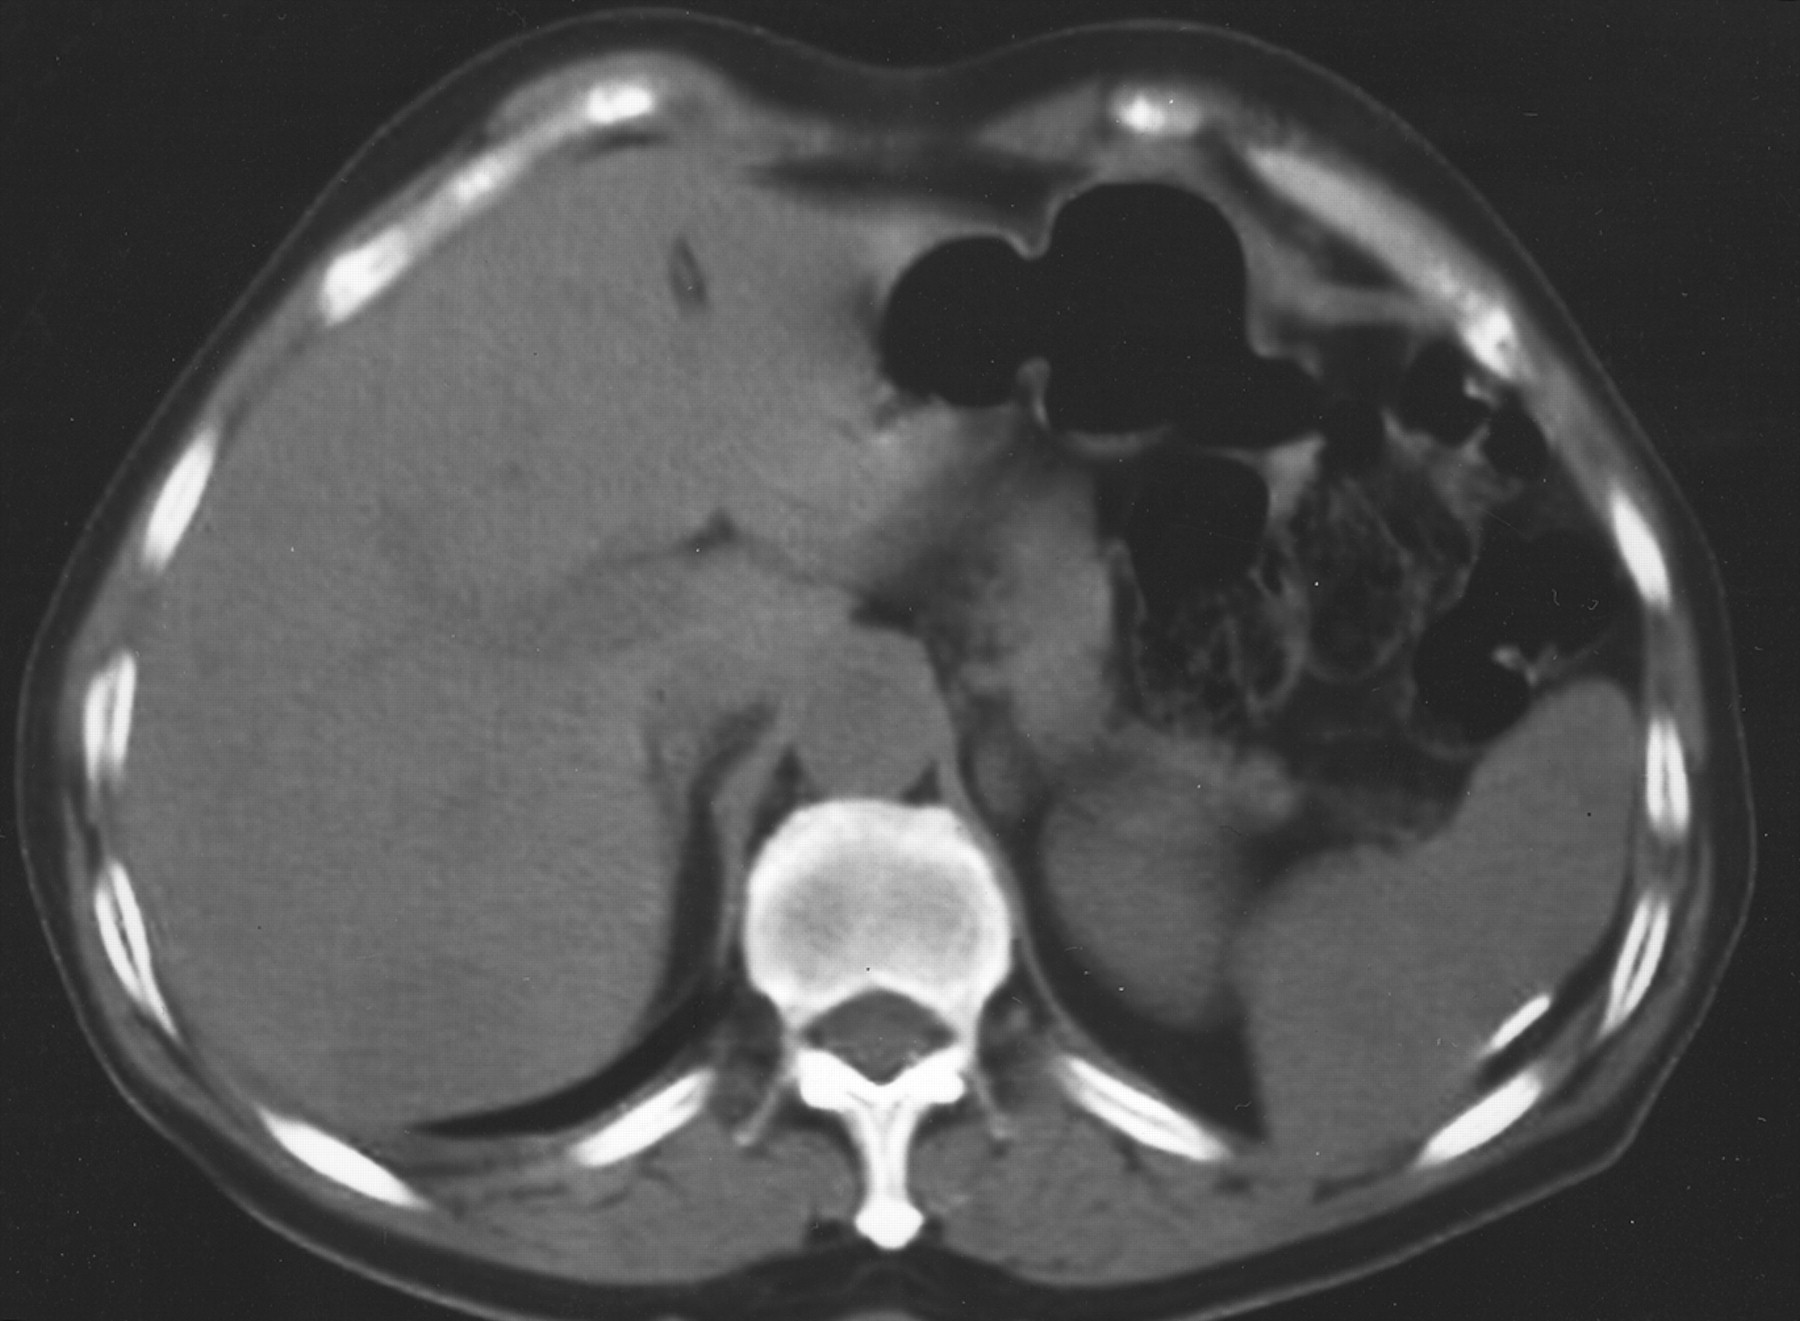
\includegraphics[width=0.48\textwidth]{images/fig1a.jpeg}
    \hfill
    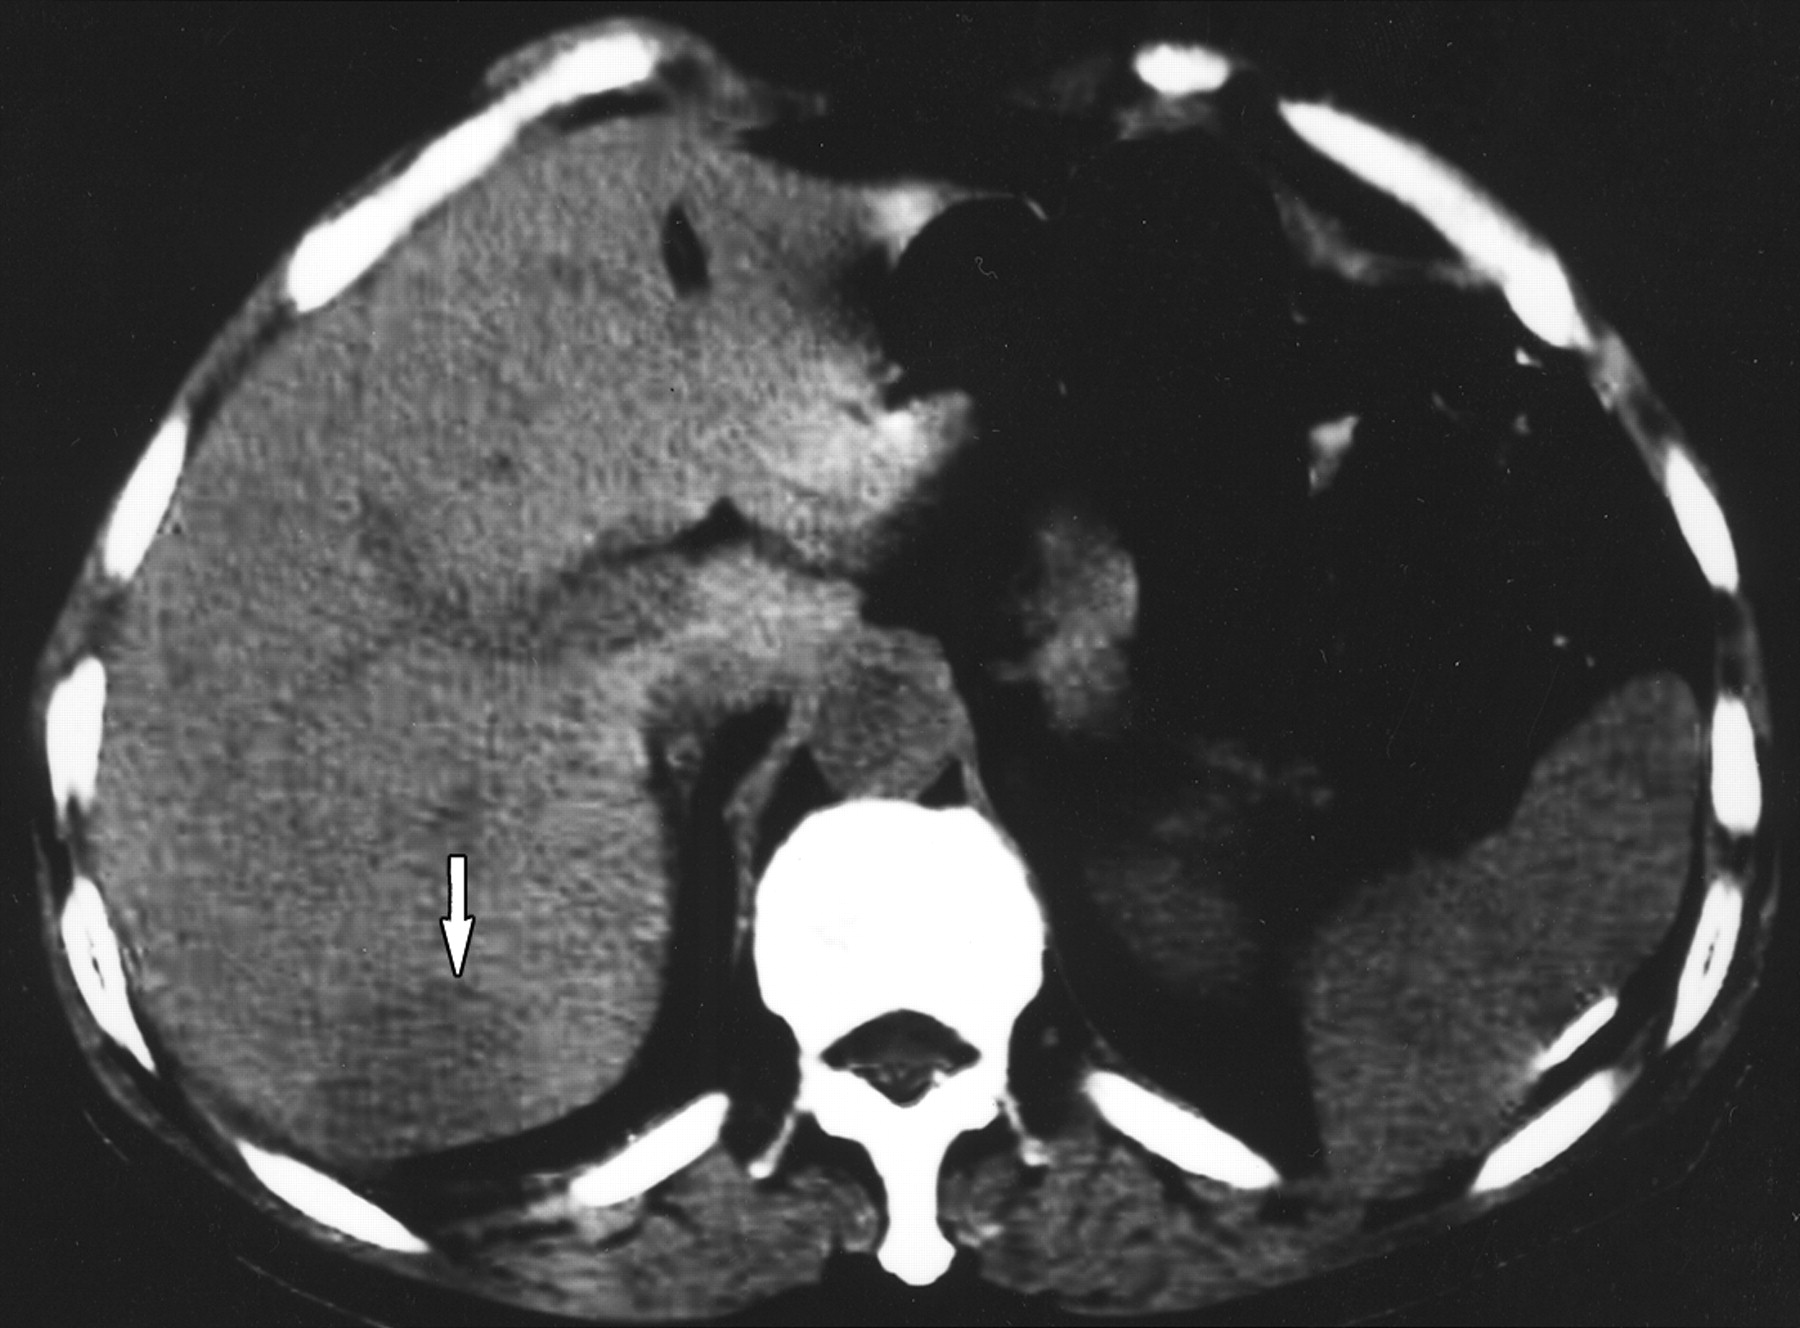
\includegraphics[width=0.48\textwidth]{images/fig1b.jpeg}
    \vspace{0.2cm} \\
    \footnotesize{شکل ۵ - تأثیر اعمال \lr{Windowing} در سی‌تی اسکن. سمت راست (بدون تنظیمات خاص) و سمت چپ (تنظیمات \lr{Liver Window}) که تومور کبدی (فلش) در آن نمایان است.}
    
\end{center}



\end{stepbox}
